%begin_custom_header
\documentclass[11pt]{article}	% RECOMB: "at least 11 point font size on U.S. standard 8 1/2 by 11 inch paper with no less than one inch margin all around."				
\usepackage[utf8]{inputenc}   % umlauts etc.
\usepackage[english]{babel}
\usepackage [autostyle, english = american]{csquotes}
\MakeOuterQuote{"}
\usepackage{hyperref}
\usepackage{array}
% ----------------------------------
\usepackage[backend=biber,style=nature,sorting=none,url=false]{biblatex}
% url = false. There are also isbn, doi etc., similar options. 
\addbibresource{/Users/mohammedalshamrani/Downloads/School/Waldispul/Publishing/z-misc/zotero-library/my_library.bib}
% ----------------------------------
% Citation style 	biblatex stylename
% ----------------------------------
% 	ACS				chem-acs
% 	AIP				phys (*)
% 	Natur			nature
% 	Science			science
% 	IEEE			ieee
% 	Chicago			chicago-authordate
% 	MLA				mla
% 	APA				apa
% ----------------------------------
% sorting options:
% ----------------------------------
%	nty 		Sort by name, title, year.
%	nyt 		Sort by name, year, title.
%	nyvt 		Sort by name, year, volume, title.
%	anyt 		Sort by alphabetic label, name, year, title.
%	anyvt 		Sort by alphabetic label, name, year, volume, title.
%	ynt 		Sort by year, name, title.
%	ydnt 		Sort by year (descending), name, title.
%	none 		Do not sort at all. All entries are processed in citation order.
% ----------------------------------
\newcommand{\harpoon}{\overset{\rightharpoonup}}
\newtheorem{theorem}{Theorem}
\usepackage{verbatim} % multiline comment
\usepackage{graphicx}
\graphicspath{{/Users/mohammedalshamrani/Downloads/School/Waldispul/Publishing/Paper_04/fig/}}
\setlength\fboxsep{0pt} % figure border padding
\setlength\fboxrule{1pt} % figure outline
\usepackage[fleqn]{amsmath}  % also \documentclass[fleqn]{article}
\usepackage[margin=1in]{geometry}
\abovedisplayskip=0pt
\abovedisplayshortskip=0pt
\belowdisplayskip=0pt
\belowdisplayshortskip=0pt
\setlength{\mathindent}{0pt}
\usepackage{amsfonts} % for R (real numbers)
\usepackage{float}
\usepackage[font=scriptsize,labelfont=bf]{caption}

\usepackage[percent]{overpic}
\usepackage[export]{adjustbox}
% ----------------------------------
%Squeezing the Vertical White Space
%http://www.terminally-incoherent.com/blog/2007/09/19/latex-squeezing-the-vertical-white-space/
% 	THIS FIXES THE PROBLEM OF SUBSECTIONS STARTING IN A NEW PAGE
\setlength{\parskip}{0pt}
\setlength{\parsep}{10pt}
\setlength{\headsep}{0pt}
\setlength{\topskip}{0pt}
\setlength{\topmargin}{0pt}
\setlength{\topsep}{0pt}
\setlength{\partopsep}{10pt}
\usepackage[compact]{titlesec}
\titlespacing{\section}{0pt}{*2}{*2} % {left margin} {above-skip} {below-kip} , The * notation replaces the formal notation using plus/minus and etc. 
\titlespacing{\subsection}{0pt}{*1}{*1}
\titlespacing{\subsubsection}{0pt}{*1}{*1}
% ----------------------------------
\newenvironment{absolutelynopagebreak}
  {\par\nobreak\vfil\penalty0\vfilneg
   \vtop\bgroup}
  {\par\xdef\tpd{\the\prevdepth}\egroup
   \prevdepth=\tpd}
% ----------------------------------
\newcommand{\bfl}{\begin{flushleft}}
\newcommand{\efl}{\end{flushleft}}
\newcommand{\mys }{\hspace{0.1cm}}
\newcommand{\figfont}{\footnotesize}

\graphicspath{{/Users/mohammedalshamrani/Downloads/School/Waldispul/Publishing/Paper_04/fig/}}
\setlength\fboxsep{0pt} % figure border padding
\setlength\fboxrule{1pt} % figure outline
\usepackage[percent]{overpic}
\usepackage[export]{adjustbox}
%begin_custom_header
%end_custom_header
\begin{document}
%begin_custom_content
\newpage
%\section{Introduction} \label{intro}			
		%\parbox[t]{\textwidth}{At the intersection”}
		
		\begin{comment}
				\begin{figure}[h]
					%\begin{overpic}[width=0.5\textwidth,grid,tics=10]{algorithmic_workflow/algorithmic_workflow.pdf}
					%\begin{overpic}[width=16.5cm, height=15.5cm, right]{algorithmic_workflow/algorithmic_workflow_cropped.pdf}
					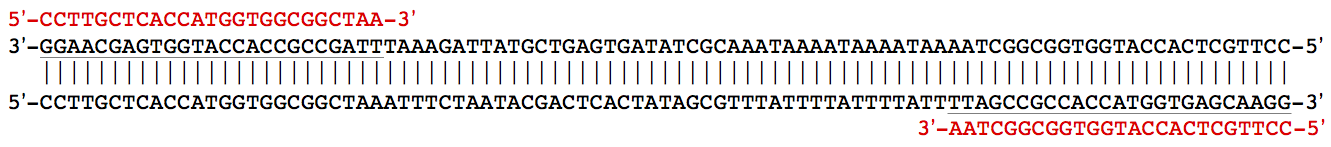
\includegraphics[scale=.5,center]{01_schematics/aseq.png} 
					%\includegraphics[scale=.3]{02.degree-dist/ER_Vinayagam.png}
					\caption{schematic}
					\label{fig:schematic}
				\end{figure}
		\end{comment}
		\begin{figure}[H]
			\begin{table}[H]
				\arrayrulecolor[HTML]{ffffff}% midrule is used to create vertical space between rows, make it white. blue = 0a84f7
				\centering
				% multirow is used to control vertical alignment within a cell: http://tex.stackexchange.com/questions/328793/table-custom-cell-vertical-alignment
				\begin{tabular}{{  | @{}p{.1cm} | p{12.5cm}@{} |   }}				
					\toprule
					\multirow{-4}{\linewidth}{\footnotesize{(1)}} & 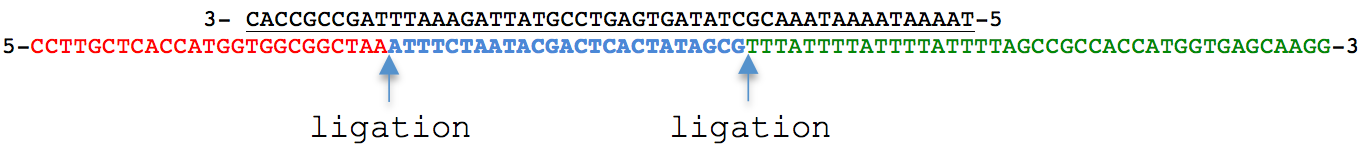
\includegraphics[scale=.25, center]{03_method/m1.png} 
					\\ \midrule\midrule\midrule\midrule  % midrule is thicker than \hline
					\multirow{-4}{\linewidth}{\footnotesize{(2)}} & 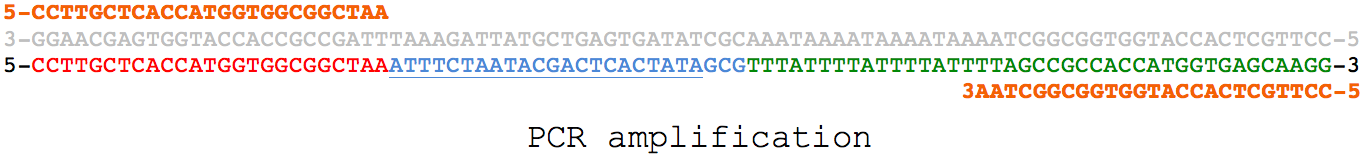
\includegraphics[scale=.25, center]{03_method/m2.png} 
					\\ \midrule\midrule\midrule\midrule  
					\multirow{-4}{\linewidth}{\footnotesize{(3)}} & 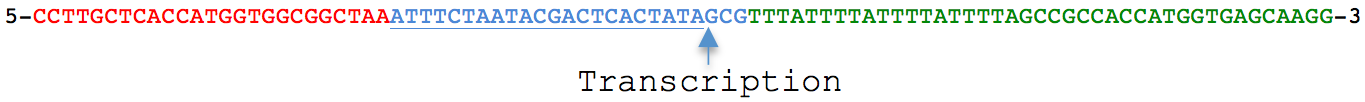
\includegraphics[scale=.25, center]{03_method/m3.png}  
					\\ \midrule\midrule\midrule\midrule  
					\multirow{-1}{\linewidth}{\footnotesize{(4)}} & 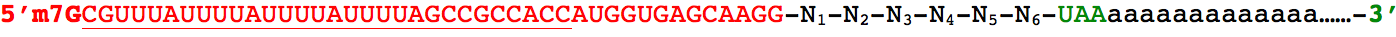
\includegraphics[scale=.25, center]{03_method/m4.png} 
					\\ \bottomrule
				\end{tabular}
			\end{table}		
			\caption{Construction of dsDNA templates}
			\label{fig:method}	
		\end{figure}

		
%end_custom_content
\printbibliography
\end{document}